\chapter{Evaluation}\label{Evaluation}
\ifpdf
    \graphicspath{{Chapter4/Chapter4Figs/PNG/}{Chapter4/Chapter4Figs/PDF/}{Chapter4/Chapter4Figs/}}
\else
    \graphicspath{{Chapter4/Chapter4Figs/EPS/}{Chapter4/Chapter4Figs/}}
\fi
A number of different clustering and classification algorithms have been used in our implementation of the event extraction system. 
Some of them are more suitable for mining social media content and some others are not. In this capter we evaluate, both quantitatively and qualitatively, 
these algorithms based on real data collected from Twitter and we provide the results of several experiments we have conducted using this dataset. 
Our quantitative analysis consists of comparing the accuracy and the quality of the clusterers and the classifers as well as their runtime performance. 
Finally, based on our results we discuss and explain which algorithms pass the test and will be used in the development of 
proof-of-concept application in Chapter \ref{CaseStudy}.

\section{Document clustering evaluation}
Cluster analysis is the core component of our system and its evaluation is of great importance to us. We have implemented 
four different clustering algorithms and some of them have been used with success in traditional document clustering. However,
in our case we are asked to tackle an entirely different problem since we deal with social media content and the challenges that come with it. 
We have identified three major challenges that are inherent to tweets and our clustering evaluation evaluates qualitatively the individual merits and demerits 
of each algorithm with respect to these challenges. More specifically, the three major challenges are:

\begin{itemize}
   \item \textbf{Number of documents:} The first difference between traditional document clustering is that our system must operate on a vast amount 
   of tweets. In March 2011 Twitter reported that a billion tweets are sent per week [put reference Penner, 2011 here] and events that are getting a lot 
   of traction, such as the Arab Spring, will be associated with a huge number of tweets. Therefore, our first consideration is scalability and whether our algorithms can cope with the 
   number of tweets.    
   \item \textbf{Document length:} Tweets, unlike normal web documents, are very short and they are limited to 140 characters. Longer documents are, in general, more likely
  to contain more examples of the features of interest than shorter ones [put reference here Hermann Moisl ] hence clustering may be more accurate with longer documents. This fact may 
  affect the accuracy of our algorithms and we should investigate their relative performance. 
   \item \textbf{Vocabulary diversity :} Another major challenge due to the nature of the tweets is the diversity of the vocabulary used. Tweets are supposed to be informal documents
   and this greatly affects the quality of their content. For example, many tweets contain spelling mistakes, typos or abbreviations and sometimes users use words from multiple languages.
   Also, usually people tend to make small modifications to existing tweets and retweet them with the consequence that we collect several tweets that essentially have the same meaning but their
   vocabulary varies. This is a big concern for us since our clustering methods use the vector space representation which uses the word frequencies to find similarities. Hence the vocabulary 
   diversity will affect the term frequencies and consequently our results. 
\end{itemize} 
What we try to achieve in the next sections is to evaluate our clustering algorithms by considering the three challenges describes above as variables. We vary these variables and 
record the performance of each algorithm in each case. In addition to these variables we also investigate the effect of different similarity measures on our results. 

   
\subsection{Data and evaluation methodology}\label{ClusteringEvaluationMethod}
Our aim is to measure the quality of a clustering algorithm and we have a few methods to choose from to achieve this. There are two categories of clustering evaluation methods and the choice depends
on whether a ground truth is available. The first category is the extrinsic methods which require the existence of a ground truth and the other category is the intrinsic methods. In general, extrinsic methods try to assign a score, $Q(C, C_g)$, to a clustering $C$, given the ground truth $C_g$, whereas intrinsic methods evaluate clustering by examining how well the clusters are separated and how compact they are [put reference data mining book here].\\\\ 
In our evaluation we decided to use an extrinsic method by constructing the ground truth using data from the Arab Spring. More specifically, we use the BCubed precision and recall metrics. The BCubed precion and recall metrics differ from the traditional precision and recall (described in section \ref{ClassifiersEvaluationMethod}) in the sense that clustering is an unsupervised learning technique and therefore we do not know the labels of the clusters beforehand. For this reason BCubed metrics evaluate the precion and recall for every example in a clustering on a given dataset according to the ground truth. The precision of an example is an indication of how many other examples in the same cluster belong to the same category as the example. The recall of an example reflects how many examples of the same category are assigned to the same cluster.\\\\ 
Formally, let $D = \{ 0_1,....,o_n \}$ be a set of examples, and $C$ be a clustering on $D$. Let $L(o_i)$ where $1 \leq i \leq n$ be the label of $o_i$ given by the ground truth, and $C(o_i)$ be the cluster identifier of $o_i$ in $C$. Then, for two examples, $o_i$ and $o_j$, where $i \neq j$, the \emph{correctness} of the relation between $o_i and o_j$ is defined by:

\begin{eqnarray}
Correctness(o_i, o_j) = \begin{cases}
                          1& \text{if $L(o_i) = L(o_j) \Leftrightarrow C(o_i) = C(o_j) $},\\
                          0& \text{otherwise}.
                        \end{cases}
\end{eqnarray} 

BCubed precision is defined as 

\begin{eqnarray}
Precision BCubed = \frac{ \sum_{i=1}^{n} \frac{\sum_{o_j:i \neq j, C(o_i)=C(o_j)}^{} Correctness(o_i, o_j)}{\Vert \{ o_j | i \neq j, C(o_i) = C(o_j)  \}  \Vert} }{n}
\end{eqnarray} 

BCubed Recall is defined as

\begin{eqnarray}
Recall BCubed = \frac{ \sum_{i=1}^{n} \frac{\sum_{o_j:i \neq j, L(o_i)=L(o_j)}^{} Correctness(o_i, o_j)}{\Vert \{ o_j | i \neq j, L(o_i) = L(o_j)  \}  \Vert} }{n}
\end{eqnarray} 
While recall and precision can be used to determine the quality of a classifier, the usual approach is to combines the recall and precision rates in a single equation and this is 
achieved using the $F$ metric which is defined as:
\begin{eqnarray}
F = \frac{2 \times precision \times recall}{precision + recall}
\end{eqnarray} 
For the construction of the ground truth we have manually labelled/categorised 300 tweets according to the events they described. These tweets are collected using our data retrieval module and they are related to the Egypt's uprising. More specifically, these tweets describe the events that took place during a 2-hour period (12pm - 14pm) on 25th of January 2011.    
    
\subsection{Results}
\subsubsection{Number of documents}
In this section we investigate the performance of the four different algorithms when the number of documents in our dataset varies while the other variables, the document length and the vocabulary diversity are kept constant. We run three different experiments for this evaluation case and in each one we change the similarity metric used. The results we obtained are illustrated in Figure \ref{DifferentSizeResults}

\begin{figure}[htbp]
  \begin{center}
    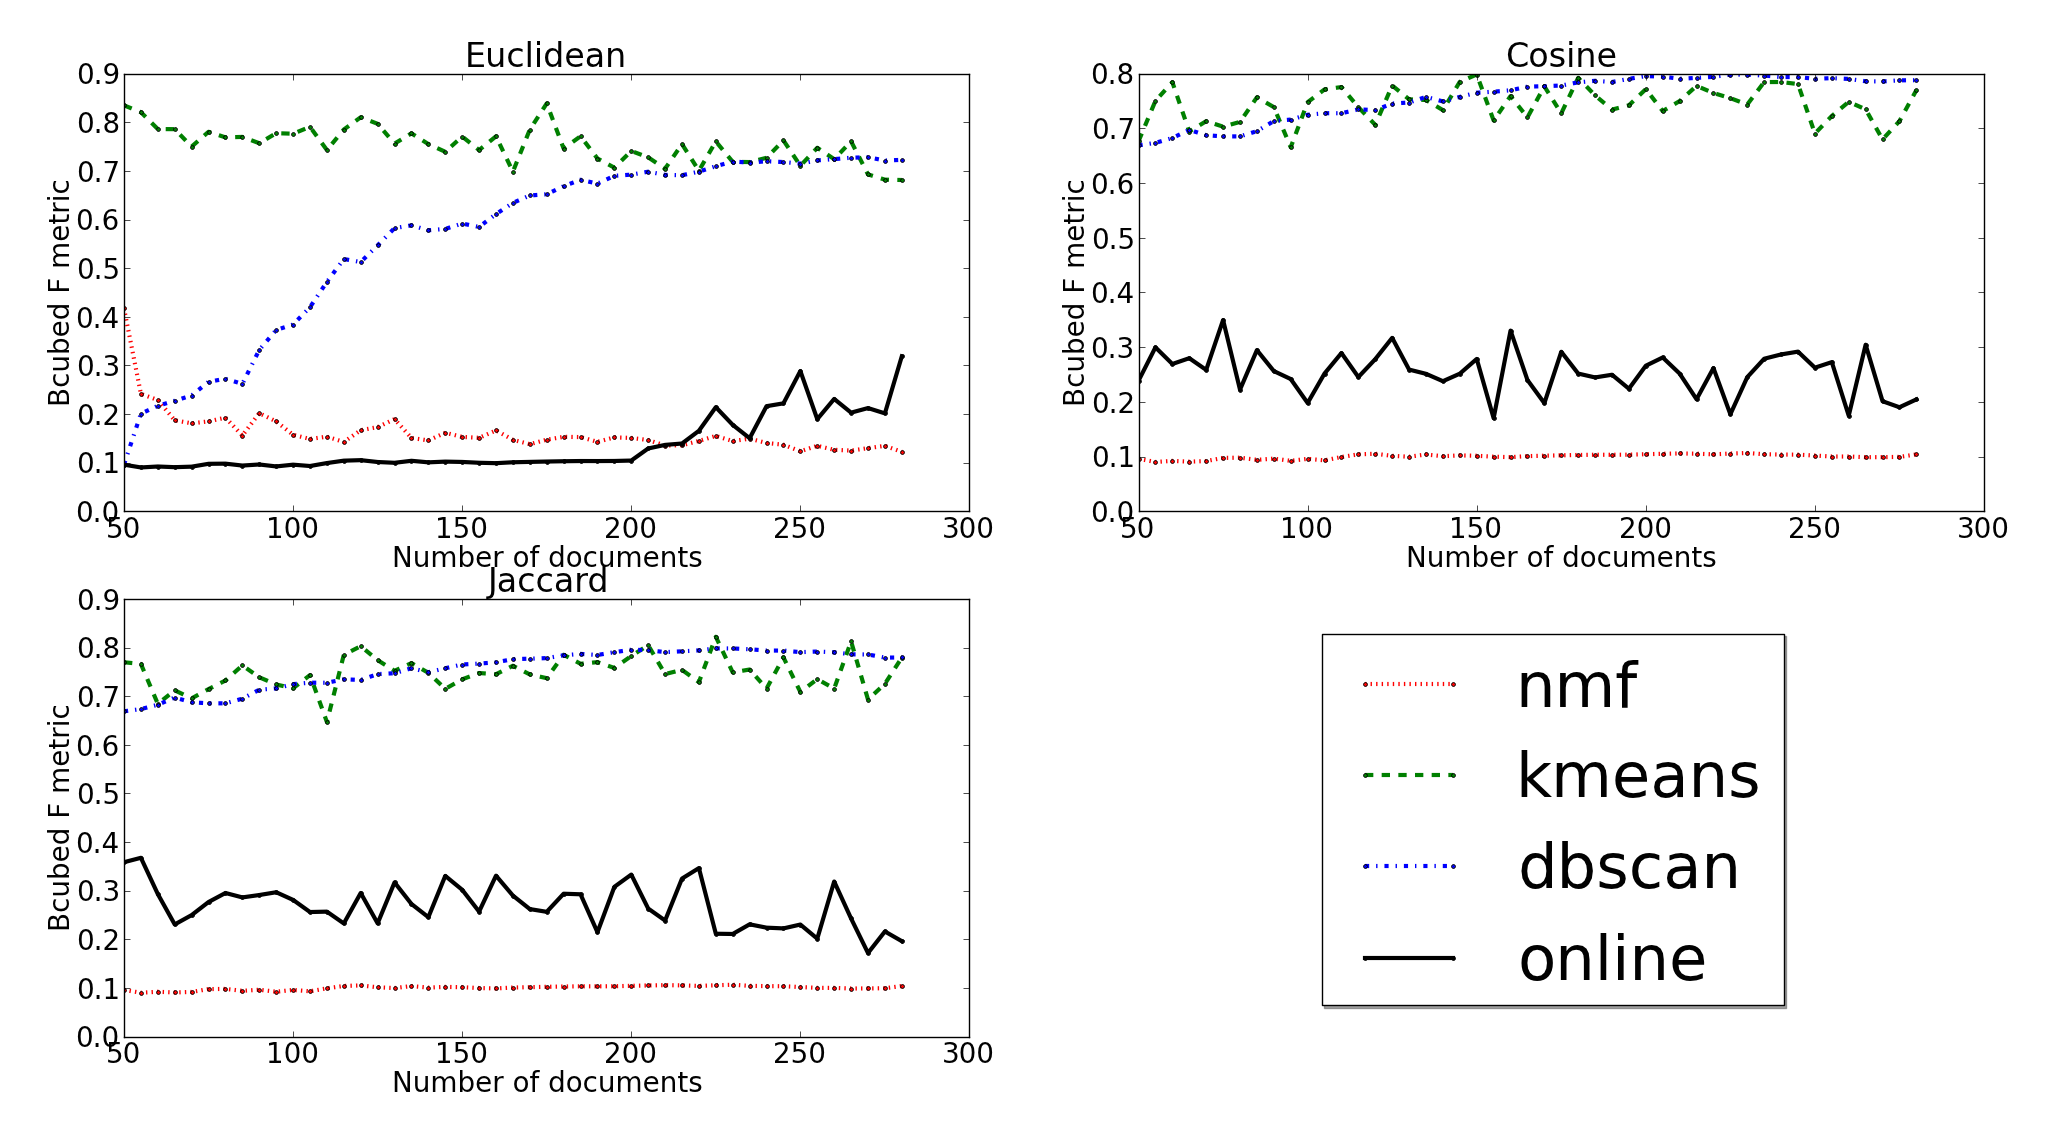
\includegraphics[height=5in, width=6in]{number_of_documents}
    \caption{Each plots depicts the results of the experiment with a different similarity measure.}
    \label{DifferentSizeResults}
  \end{center}
\end{figure}

\subsubsection{Document length}
\begin{figure}[htbp]
  \begin{center}
    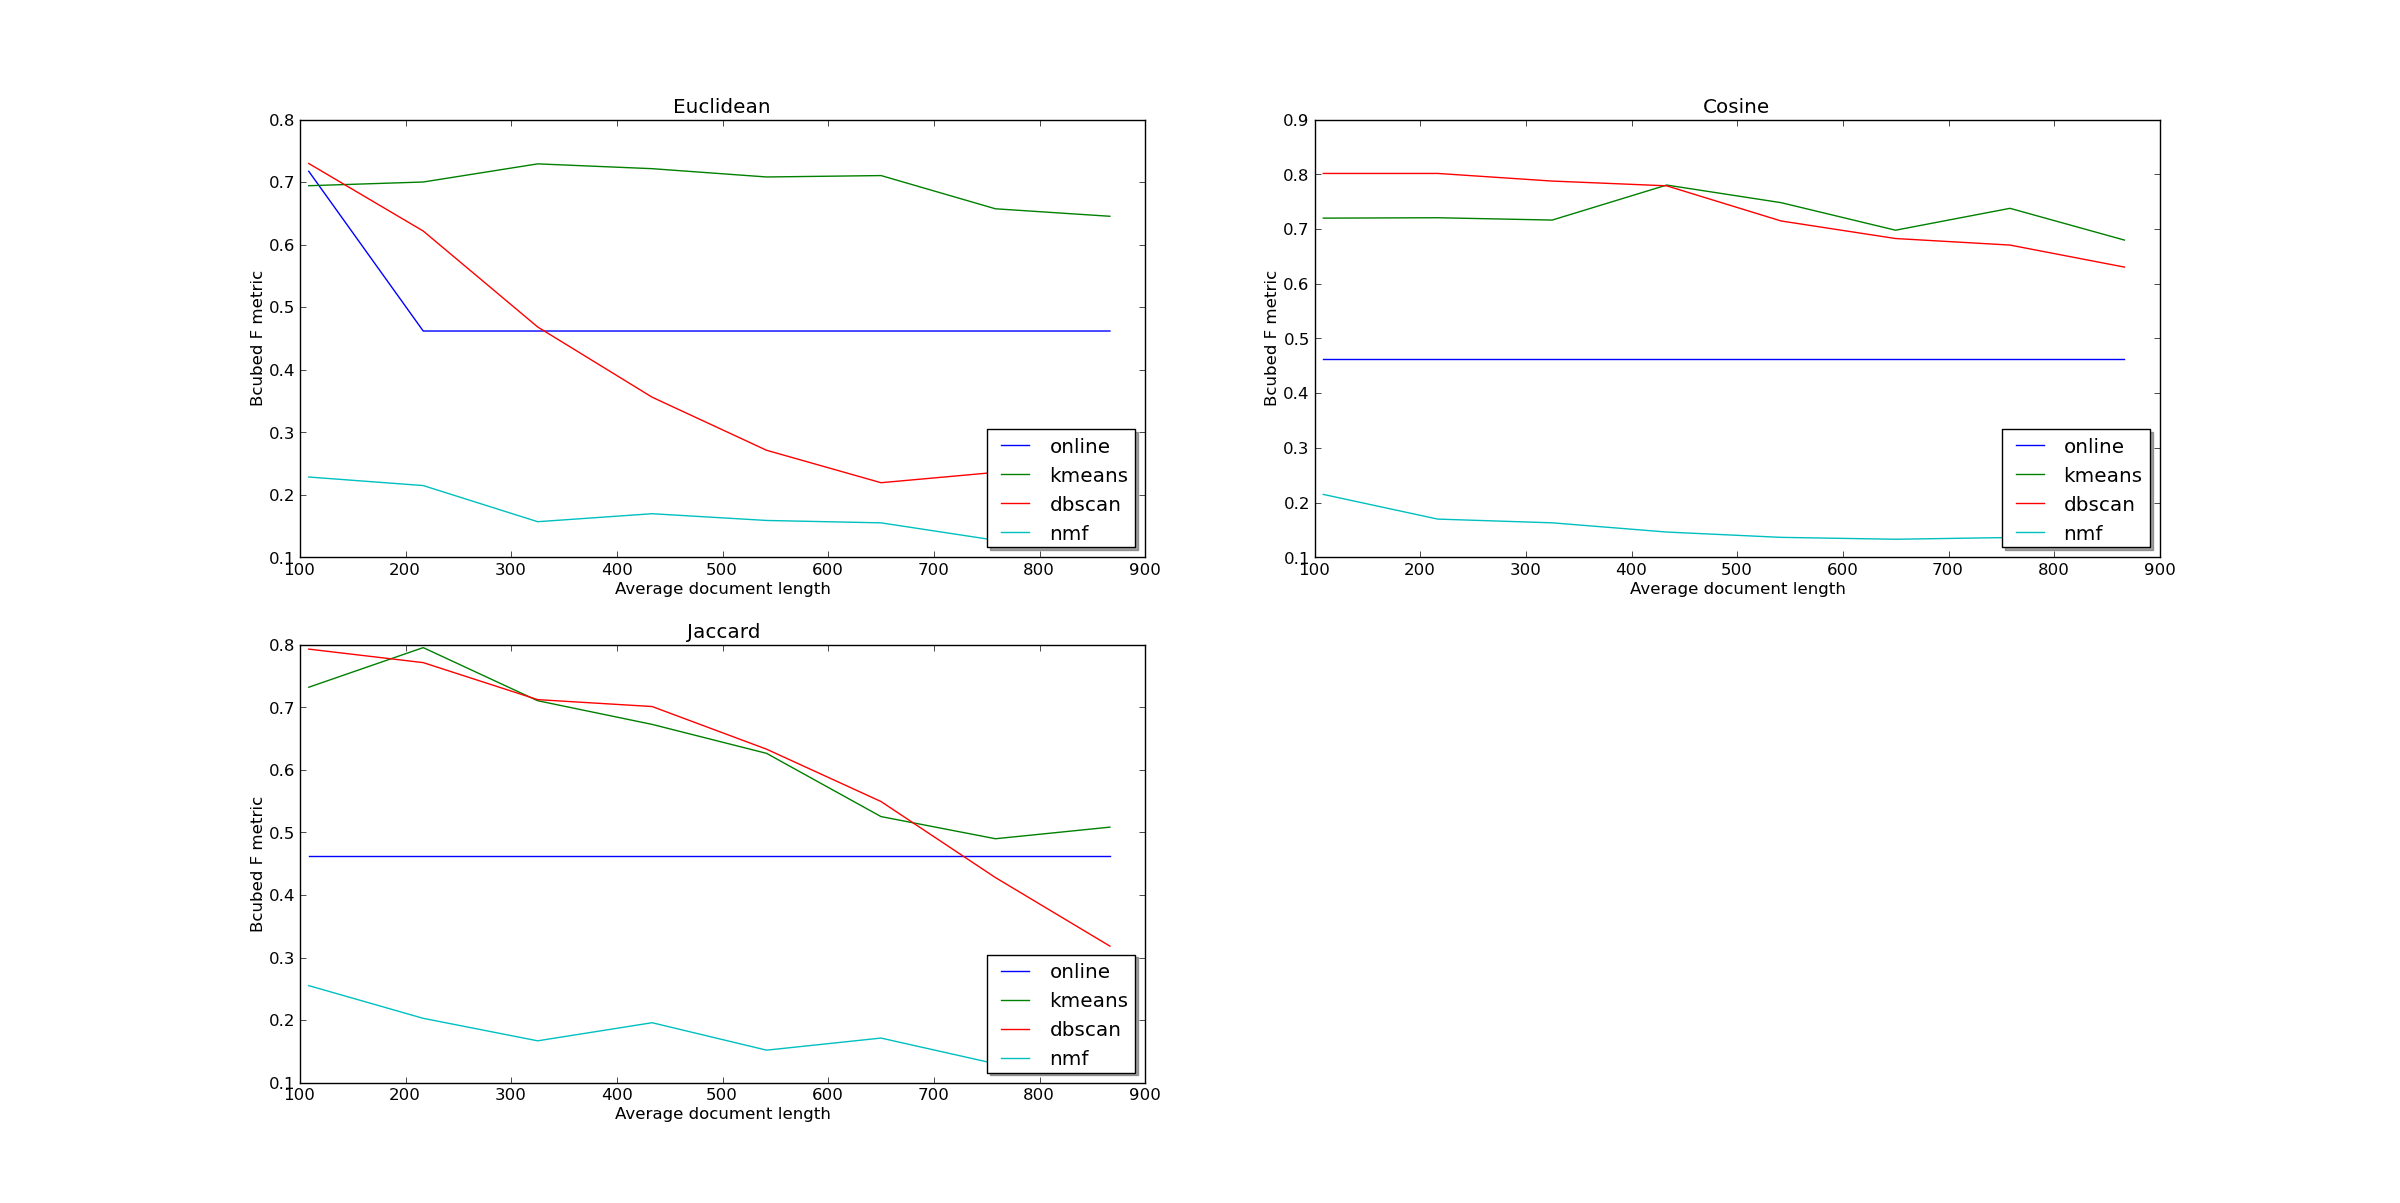
\includegraphics[height=5in, width=6in]{average_document_length}
    \caption{Each plots depicts the results of the experiment with a different similarity measure.}
    \label{DifferentLengthResults}
  \end{center}
\end{figure}

\subsubsection{Vocabulary diversity}

\begin{figure}[htbp]
  \begin{center}
    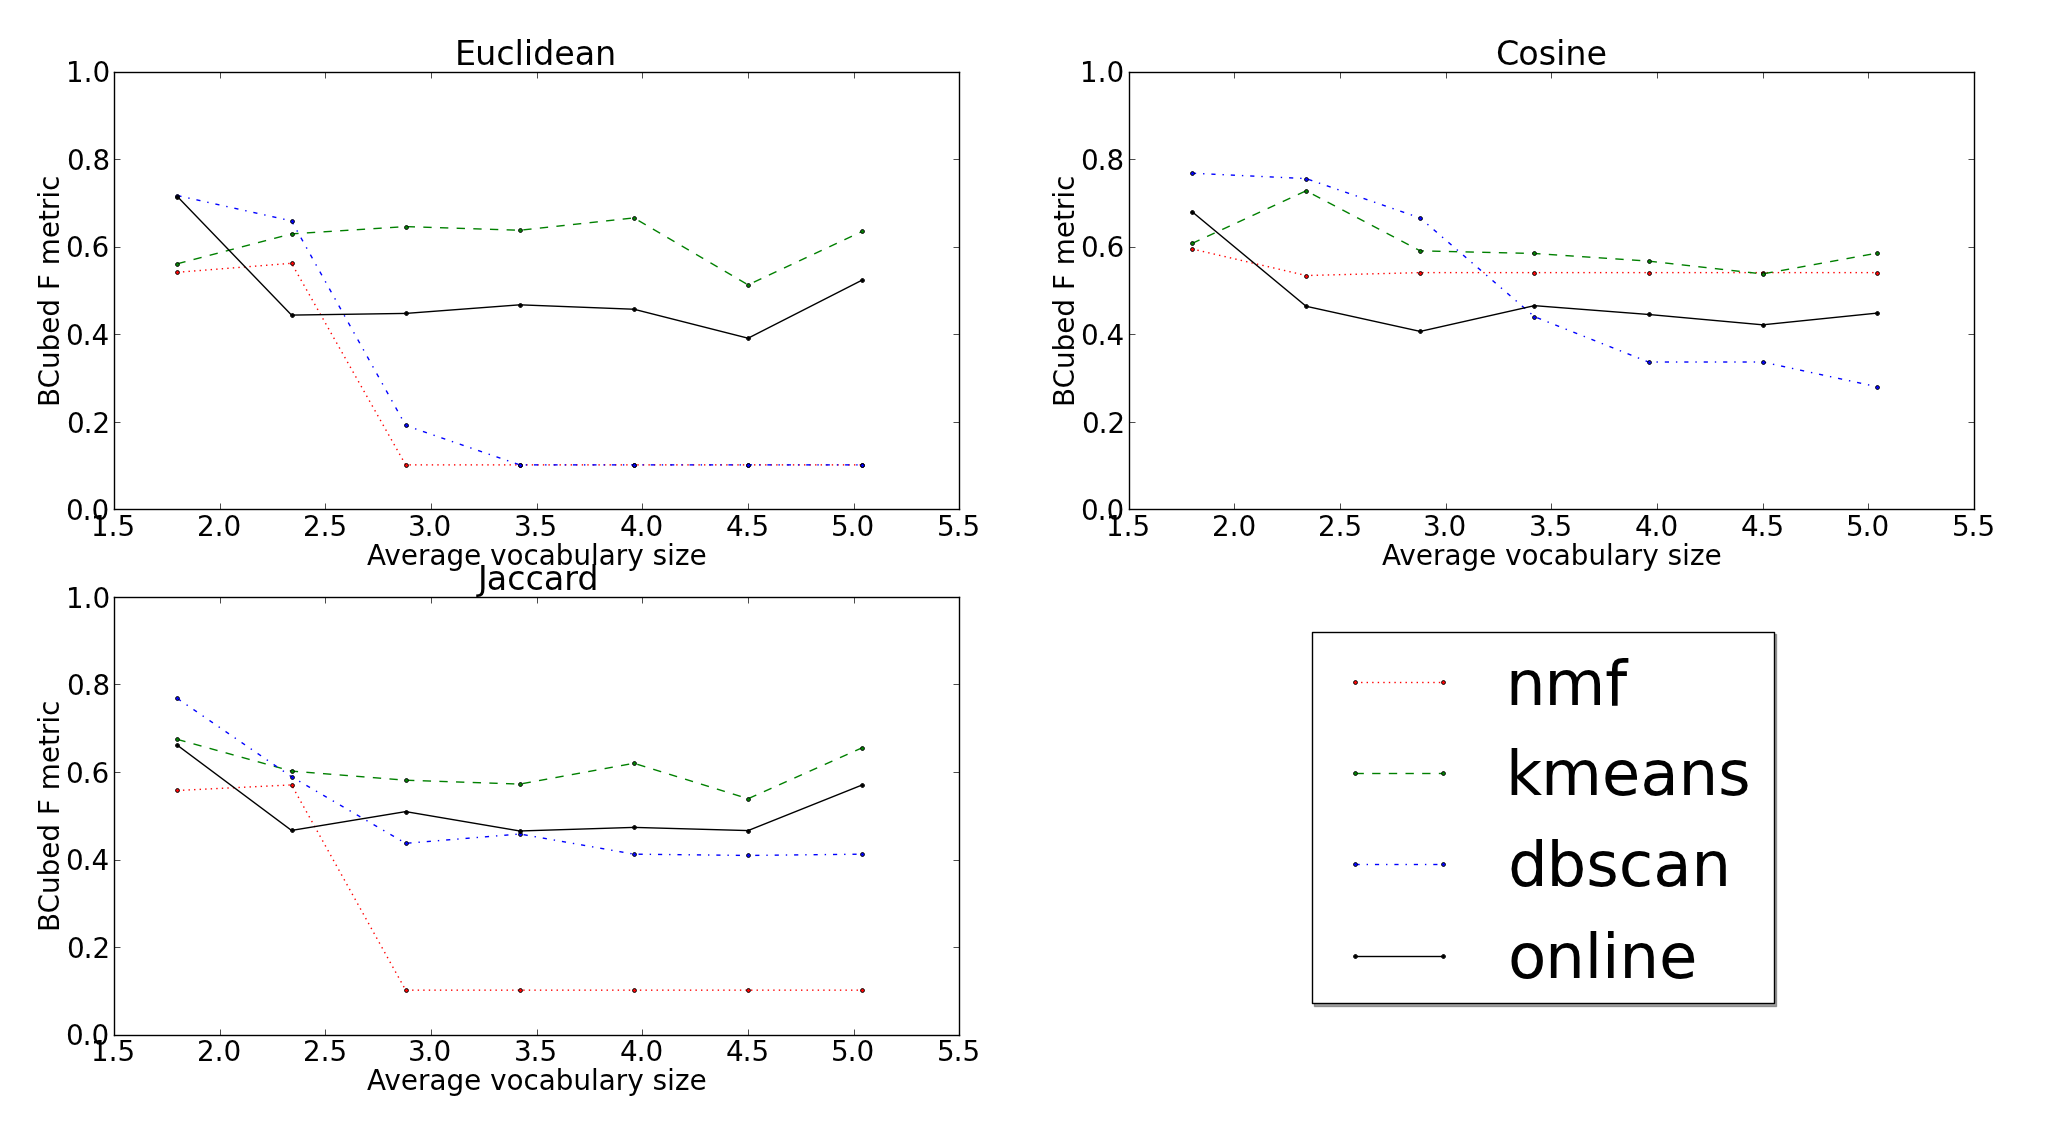
\includegraphics[height=5in, width=6in]{vocabulary}
    \caption{Each plots depicts the results of the experiment with a different similarity measure.}
    \label{DifferentVocabularyResults}
  \end{center}
\end{figure}

\subsubsection{Execution time performance}
Here I will put the results and graphs about the execution time performance of the algorithms

\section{Twitter user classification evaluation}

\subsection{Data and evaluation methodology}\label{ClassifiersEvaluationMethod}
In this section our aim is to identify which one of our classification algorithms performs better in terms of classification accuracy. Our classifier evaluation process involves the precision and recall metrics as well as the $F_1$ score. The precision and recall metrics definitions in this section are different from the ones described in section \ref{ClusteringEvaluationMethod} since classification is a supervised learning method and we can calculate these metrics using the labels of that training dataset. More specifically, precision can be thought as a measure of what percentage of examples that are classified by a classifier in a certain class are actually members of that class. On the other hand recall is a measure of what percentage of the overall population of examples belonging to a certain class have been classified by the classifier in that particular class. Formally, precision and recall are defined as:

\begin{eqnarray}
precision = \frac{TP}{TP + FP}
\end{eqnarray}  

\begin{eqnarray}
recall = \frac{TP}{TP + FN}
\end{eqnarray}  

where 

\begin{itemize}
  \item True Positives ($TP$): These are the positive tuples that were correctly labelled by our algorithm. 
  \item True Negatives ($TN$): These are the negative tuples that were correctly labelled by our algorithm.
  \item False Positives ($FP$): These are the negative tuples that were incorrectly labelled as positive by our algorithm.
  \item False Negatives ($FN$): These are the positive tuples that were incorrectly labelled as negatives by our algorithm.
\end{itemize}\vspace{15pt}

\subsection{Results and discussion}

\begin{figure}[htbp]
  \begin{center}
    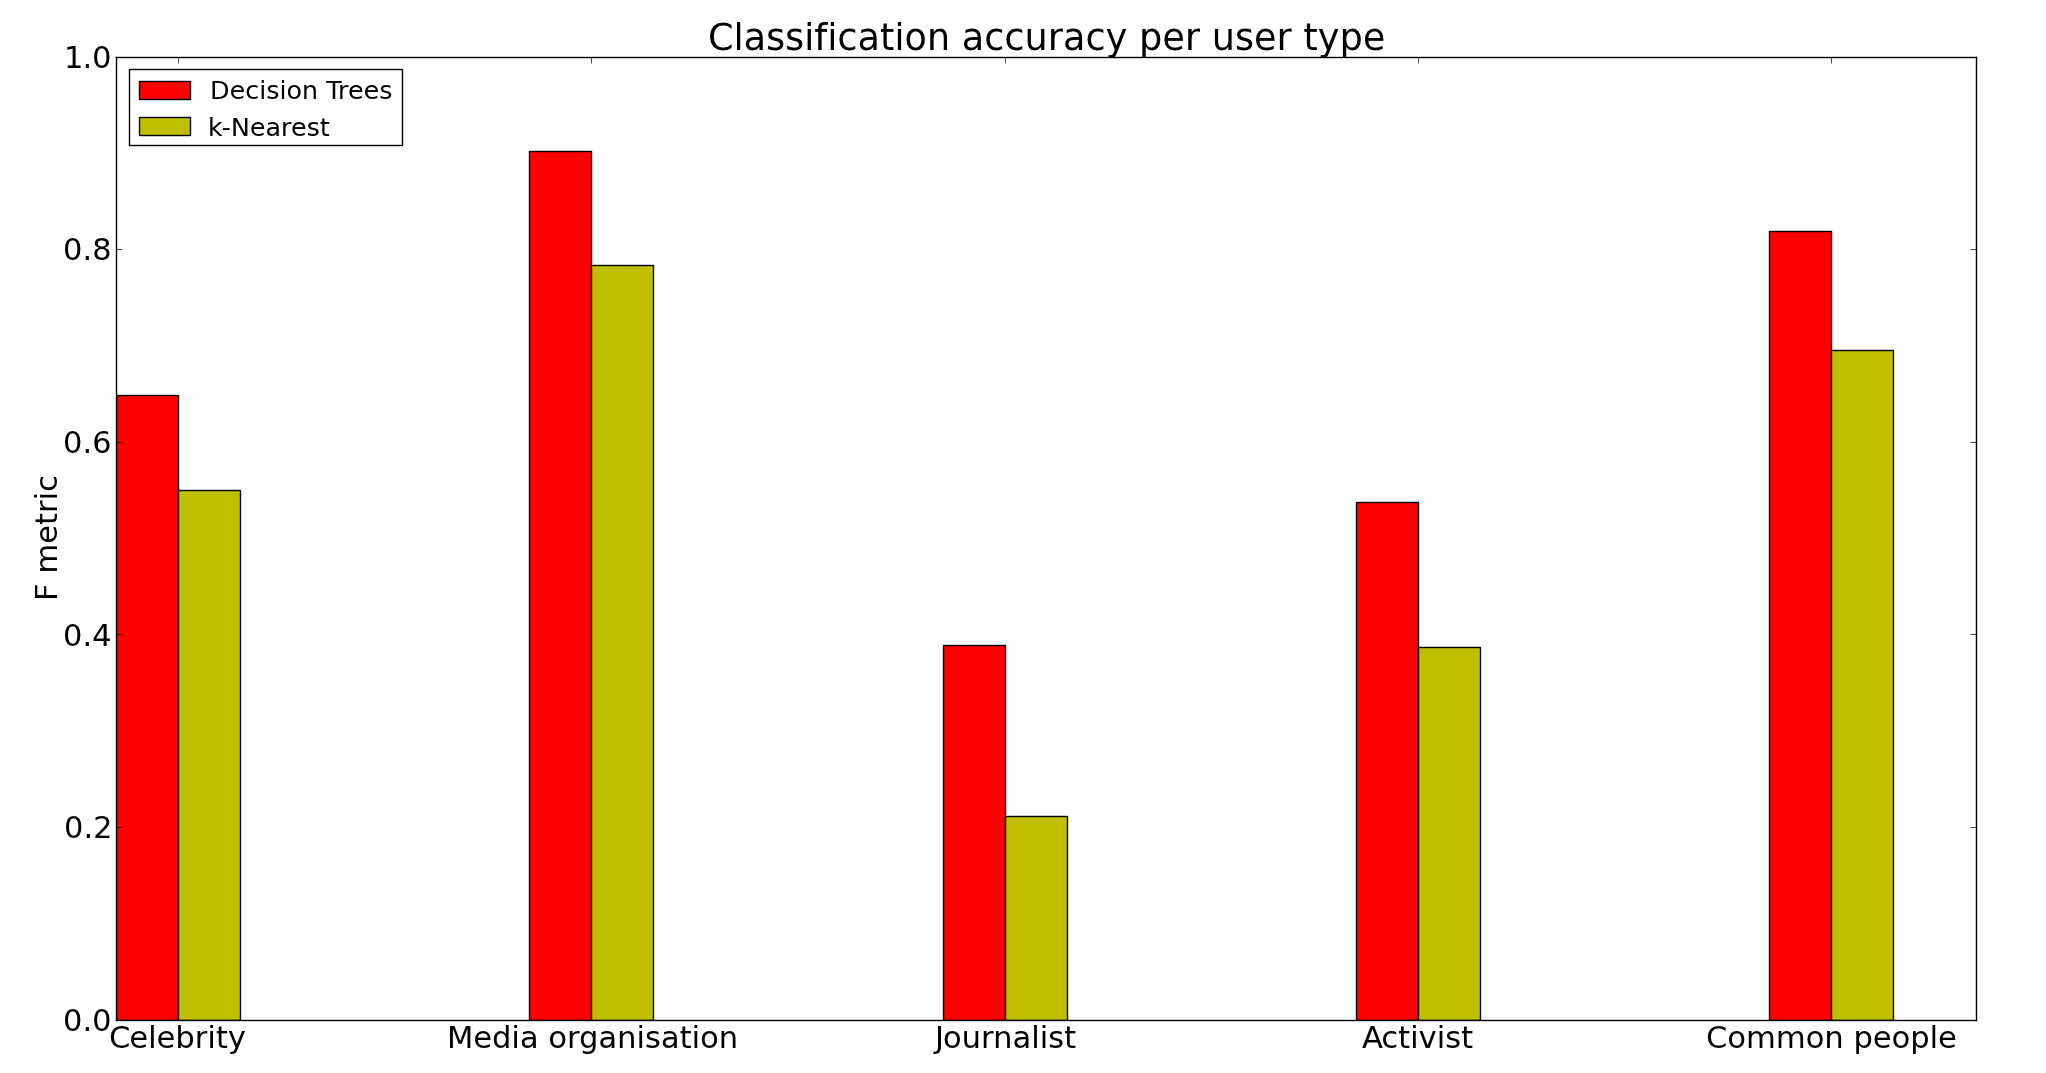
\includegraphics[height=5in, width=6in]{classifiers}
    \caption{The F metrics obtain after 10-fold cross validation on our dataset for the two classifiers.}
    \label{DifferenClassifiersResults}
  \end{center}
\end{figure}


\section{Optimisations}
Briefly explain how we improbed the execution time

\section{Summary}

% ------------------------------------------------------------------------


%%% Local Variables: 
%%% mode: latex
%%% TeX-master: "../thesis"
%%% End: 
